% This is samplepaper.tex, a sample chapter demonstrating the
% LLNCS macro package for Springer Computer Science proceedings;
% Version 2.20 of 2017/10/04
%
\documentclass[runningheads]{llncs}
%
\usepackage{float}
\usepackage{natbib}
\usepackage{amsfonts}
\usepackage{amsmath, bm}
\usepackage{booktabs} % For pretty tables
\usepackage{caption} % For caption spacing
\usepackage{subcaption} % For sub-figures
\usepackage{graphicx}
\usepackage{pgfplots}
\usepackage[all]{nowidow}
\usepackage[utf8]{inputenc}
\usepackage{tikz}
\usetikzlibrary{er,positioning,bayesnet}
\usepackage{multicol}
% \usepackage{algpseudocode,algorithm,algorithmicx}
\usepackage[ruled,vlined]{algorithm2e}
\usepackage{algpseudocode,algorithmicx}
% \usepackage{minted}
\usepackage{hyperref}
\usepackage[inline]{enumitem} % Horizontal lists
% Used for displaying a sample figure. If possible, figure files should
% be included in EPS format.
%
% If you use the hyperref package, please uncomment the following line
% to display URLs in blue roman font according to Springer's eBook style:
% \renewcommand\UrlFont{\color{blue}\rmfamily}

\newcommand{\card}[1]{\left\vert{#1}\right\vert}
\newcommand*\Let[2]{\State #1 $\gets$ #2}
\definecolor{blue}{HTML}{1F77B4}
\definecolor{orange}{HTML}{FF7F0E}
\definecolor{green}{HTML}{2CA02C}

\pgfplotsset{compat=1.14}

\renewcommand{\topfraction}{0.85}
\renewcommand{\bottomfraction}{0.85}
\renewcommand{\textfraction}{0.15}
\renewcommand{\floatpagefraction}{0.8}
\renewcommand{\textfraction}{0.1}
\setlength{\floatsep}{3pt plus 1pt minus 1pt}
\setlength{\textfloatsep}{3pt plus 1pt minus 1pt}
\setlength{\intextsep}{3pt plus 1pt minus 1pt}
\setlength{\abovecaptionskip}{2pt plus 1pt minus 1pt}

\begin{document}
%
\title{Approximate Bayesian Computation Overview}
%
%\titlerunning{Abbreviated paper title}
% If the paper title is too long for the running head, you can set
% an abbreviated paper title here
%
\author{Davi Sales Barreira}
%
%\authorrunning{F. Author et al.}
% First names are abbreviated in the running head.
% If there are more than two authors, 'et al.' is used.
%
\institute{FGV - Escola de Matemática Aplicada, Rio de Janeiro, Brasil\\ 
\email{davisbarreira@gmail.com}}
%
\maketitle              % typeset the header of the contribution
%
\begin{abstract}
Approximate Bayesian Computation (ABC)
methods are known as likelihood-free techniques, thus are a useful
approach in problems that the likelihood is intractable, e.g., likelihood
not available in closed form, or likelihood too expensive to calculate.
In this article, we present an overview of the method by replicating
the paper Approximate Bayesian computational
methods by \cite{Marin2012}.

\keywords{Approximate Bayesian Computation \and likelihood-free \and
Monte Carlo.}
\end{abstract}
%
%
%
\section{Introduction}
\subsection{Original ABC} \label{subsec:statistical-summaries}

The Approximate Bayesian Computation method was originally described
by \citet{Rubin1984} as a thought experiment to explain how to sample
from a posterior distribution with a frequency interpretation.
The method became proeminent due to the fact that it circumvents
the need to calculate the likelihood function in order to
obtain the posterior distribution. This can be a very useful
feature in scenarios where the likelihood is intractable or
too expensive to calculate. One example is in the case where
one has latent variables, thus, the likelihood is expressed as:

\begin{equation}
  \ell(\bm\theta \mid \bm y) =
  \bm\int \ell^*(\bm\theta \mid \bm y, \bm u) d\bm u
\end{equation}
with $\bm y$ being the observed variable,
$\bm u$ the latent variable and $\bm\theta$ is the parameter of interest.

\citet{Tavare505} introduced the ABC algorithm as a rejection
techinique to obtain the posterior distribution without the explicit
calculation of the likelihood. This original algorithm is given below.

\begin{algorithm}[H]
\SetAlgoLined
\For{i=1 to N}{
 \Repeat{$\bm y = \bm z$}{
    Sample $\bm\theta' \sim \pi(\cdot)$

    Generate $\bm z \sim p(\cdot \mid \bm\theta')$
 }
  
}
 \caption{Original ABC method}
\end{algorithm}

The proof that the algorithm indeed results in an iid sample
from the posterior is shown below. Let $\bm y$ be the observed,
$\bm \theta$ the parameter of interest and $\bm z$ the generated
samples.

\begin{equation}
  f(\bm \theta_i) \propto \sum_{\bm z \in \mathbb{D}}
  \pi(\bm \theta_i) p(\bm z \mid \bm \theta_i) \mathbb I_{\bm y}(\bm z)
  = \pi(\bm \theta_i) p(\bm y \mid \bm \theta_i) \propto
  \pi(\bm \theta_i \mid \bm y)
\end{equation}

The original ABC formulation only works for
the case where $\bm y$ is discrete
taking finite values, and therefore, an exact match is possible
to be obtained in a finite number of simulations. \citet{Pritchard1999}
then extended the method to a more general form considering an
approximation instead of an exact match. This extended algorithm is
shown below, where

\begin{itemize}
  \item[--] $\eta$ is a function defining a statistic (e.g. the mean),
  \item[--] $\rho$ is a distance function,
  \item[--] $\epsilon$ is an acceptance tolerance.
\end{itemize}

\begin{algorithm}[H]
\SetAlgoLined
\For{i=1 to N}{
 \Repeat{$\rho[\eta(\bm y) , \eta (\bm z)] \leq \epsilon$}{
    Sample $\bm\theta' \sim \pi(\cdot)$

    Generate $\bm z \sim p(\cdot \mid \bm\theta')$
 }
  
}
 \caption{ABC method for discrete and continuous distributions}
\end{algorithm}

For this ABC algorithm, instead of the actual posterior,
we get

\begin{equation}
\pi_\epsilon(\bm \theta, \bm z \mid \bm y) = 
\frac{\pi(\bm \theta) p(\bm z \mid \bm \theta)
\mathbb I_{A_{\epsilon,\bm y}}(\bm z)}
{\int_{A_{\epsilon,\bm y}\times \bm\theta}\pi(\bm \theta)
p(\bm z \mid \bm \theta)d\bm z d \bm \theta}
\end{equation}
where, $A_{\epsilon,\bm y} = \{
\bm z \in \mathcal D \mid \rho[\eta(\bm z), \eta(\bm y) \leq \epsilon]
\}$.
Hence, for a tolerance ($\epsilon$) "small enough", we expect a good
approximation of the real posterior.
\begin{equation}
\pi_\epsilon(\bm \theta \mid \bm y) = 
\int \pi_\epsilon(\bm \theta, \bm z \mid \bm y) d \bm z \approx
\pi(\bm \theta \mid \bm y)
\end{equation}


\subsection{Moving Average} \label{subsec:statistical-summaries}

We will use the Moving Average model, also denoted as MA(q),
for assessing the performance of the ABC methods. The MA(q) process
is a stochastic process defined by:

\begin{equation}
y_k = u_k + \sum_{i=1}^q \theta_i u_{k-i}
\end{equation}
where $(u_k)_{k \in \mathbb Z} \overset{iid}{\sim} N(0,1)$.
The true posterior distribution of MA(2) and MA(1) models can be
numerically computed, since the likelihood function is indeed avaliable.
Therefore, the approximations obtained through ABC can be compared with
the true posterior. The marginal posterior distributions are also
obtained numerically.

For $q=2$, imposing the standard identifiability condition
we obtain the following conditions:

\begin{equation}
-2 < \theta_1 < 2, \quad \quad \theta_1+\theta_2 > -1, \quad \quad
\theta_1 - \theta_2 < 1.
\end{equation}
hence, we use an uniform distribution over this triangular region as
prior for $\bm \theta$.

We generate a synthetic sample of length 100 using
$(\theta_1, \theta_2) = (0.6, 0.2)$. For $q=2$, the 
true posterior has the following form:
\begin{equation}
\pi(\bm\theta \mid \bm y) \propto \pi(\bm\theta)
p(\bm y \mid \bm \theta), \quad \quad
\bm y \mid \bm \theta \sim MVN(0, \Sigma) \quad
\end{equation}

$$
\Sigma =
\left[ 
\begin{smallmatrix}
 1+\theta_1^2 + \theta_2^2    & \theta_1 + \theta_2 \theta_1 & \theta_2                     & 0                            & 0        & 0 & ... & 0 \\
 \theta_1 + \theta_2 \theta_1 & 1+\theta_1^2 + \theta_2^2    & \theta_1 + \theta_2 \theta_1 & \theta_2                     & 0        & 0 & ... & 0 \\
 \theta_2                     & \theta_1 + \theta_2 \theta_1 & 1+\theta_1^2 + \theta_2^2    & \theta_1 + \theta_2 \theta_1 & \theta_2 & 0 & ... & 0 \\
 0               & \theta_2   & \theta_1 + \theta_2 \theta_1 & 1+\theta_1^2 + \theta_2^2    & \theta_1 + \theta_2 \theta_1 & \theta_2 &... & 0 \\
 \vdots & \vdots & \vdots & \vdots & \vdots & \vdots & \vdots & \vdots \\
 0 & 0 & 0 & 0 & 0 & \theta_2 & \theta_1 + \theta_1\theta_2 & 1+\theta_1^2 + \theta_2^2 \\
\end{smallmatrix}
\right]
$$

For this model, applying the ABC algorithm consisted in the
following steps:
\begin{itemize}
  \item Sample $\bm \theta ^ *$ from the uniform triangular prior
  using rejection sampling;
  \item For each $k \in \{-1,0, 1, ..., 100 \}$, sample
  $u_k \overset{iid}{\sim} N(0,1)$.
  \item For each $k \in \{ 1, 2, ..., 100\}$, calculate 
  $z_k = u_k + \sum^2_{i=1}\theta_i^* u_{k-i}$.
\end{itemize}

Two distance metrics were initially compared.
The raw distance between the series

\begin{equation}
\rho^2\{ \bm z, \bm y\} = \sum^{n=100}_{k=1}(y_k - z_k)^2
\end{equation}
and the sum of the quadratic distances between the first $q = 2$
autocovariances.
\begin{equation}
\tau_j(\bm x) = \sum^{n=100}_{k = j+1} x_k x_{k-j}, \quad \quad
\rho^2 = \sum^{q=2}_{j=0}(\tau_j(\bm y) - \tau_j(\bm z))^2
\end{equation}

Below we present the results of running ABC for the MA(2) process
using the autocovariances distance.

  \begin{figure}[H]
      \centering
      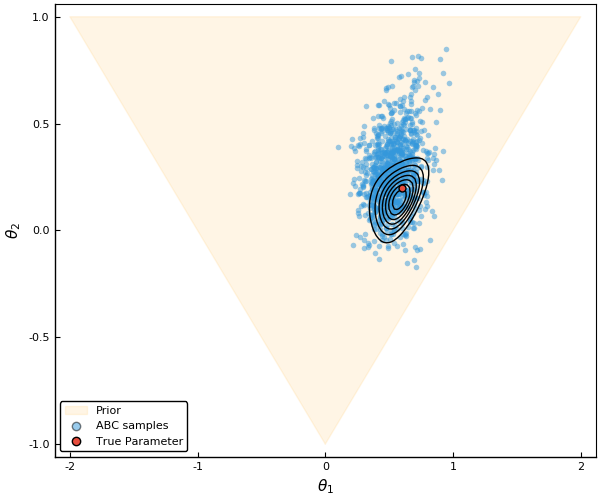
\includegraphics[width=10cm]{images/ABCmodel1.png}
      \caption{Comparison between the true posterior
      (\textit{line in black}), with the samples produced using the ABC
      . The number of simulations is $N = 10^6$,
      and the threshold $\epsilon$ corresponds to the quantile of
      accepting 0.1\%. The $\rho$ used was the distance
      of the autocovariances.}
  \end{figure}

\section{ABC Calibration}
\subsection{Summary Statistics ($\eta$)}
\label{subsec:statistical-summaries}

As the number of observations
grow, using the raw distance between each observation becomes too
prohibitive, due to the rarity of actually
obtaining samples close to each observation.
The alternative is to try using summary statistics of low dimension.
The ideal case is using sufficient statistics, which guarantee that the
method indeed approximates the true posterior.
The problem is that
low-dimensional sufficient statistics are rarely available. Hence,
choosing an appropriate low-dimensional statistic is paramount for
obtaining good approximations with ABC \citep{Marin2012}.

\citet{Beaumont2018} separates the approaches to address this
problem into two categories: one is optimally choosing
subsets of summary statistcs, and the other is projecting
a set of summary statistics onto lower dimensional maps.

In the first category, \citet{Joyce2008} introduced the concept
of approximate sufficiency. The main idea is that given a set
of summary statistics $s \subset S$, an approximately sufficient subset can
be found by sequantially including those statistics into the ABC
target. The method develops a score written as
\begin{equation}
\delta_k = sup_\theta \{
\log f(s_k \mid s_1,...,s_{k-1},\theta)
\}
- inf_\theta\{
\log f(s_k \mid s_1,...,s_{k-1},\theta)
\}
\end{equation}
and tests whether $\delta_k$ is less than a given tolerance. In the
case this is true, the statistic is deemed approximately sufficient.

\citet{Marin2012} present some reservations regarding this method.
They state that the construction of the statistics is not
discussed in the paper by \citet{Joyce2008}. Secondly, the
order in which the statistics are tested may alter the final subset.
And finally, that the corrections proposed do not address the impact
of correlation between the summary statistics.

In the second category,
\citet{fearnhead2010constructing} propose a way of constructing
appropriate summary statistics for ABC in a semiautomatic manner.
Their method aims at minimizing the expected posterior loss
\begin{equation}
\mathbb E[(\bm\theta - \bm{\hat\theta})\mid \bm y]
\implies
\bm {\hat\theta} = \mathbb E[\bm\theta \mid \bm y]
\end{equation}
hence, the optimal summary statistic is
\begin{equation}
s = \mathbb E[\bm \theta \mid \bm y]
\end{equation}
Since $E[\bm \theta \mid \bm y]$ is unknown, it can instead
be estimated by performing a linear regression on each
component of $\bm \theta$. Therefore, the single optimal
summary statistic is written as
\begin{equation}
s_{opt} =  \beta^T f(s)
\end{equation}
where $\beta$ is the vector of the regression coefficients and
$f(s)$ is the vector of summary statistics functions.


\subsection{Tolerance threshold($\epsilon$)}
\label{subsec:statistical-summaries}
The choice of $\epsilon$ is mostly driven by computational
limitations. The lower the value of $\epsilon$, the higher
the number of simulations required. The standard practice
\citep{Beaumont2012} is to chose $\epsilon$ as a quantile
of the simulated distances $\rho$, e.g., for $10^6$ simulations,
taking $\epsilon = 0.1\%$ corresponds to accepting
$10^3$ sampled $\bm \theta$'s. This implies that the choice
of $\epsilon$ is just a proxy for the number of simulations
to be performed.

\subsection{Calibration comparison in MA(2)}
\label{subsec:statistical-summaries}

Using the MA(2) model, we run the ABC algorithm comparing
different calibrations. As stated before, two different
summary statistics are used, the raw distance and the
autocovariances distances. Figure ~\ref{fig:calibration1}
makes it clear that
the autocovariances distances perfom better that the raw distances,
therefore, through the rest of this article we will only be using
the autocovariances distances.

Figure ~\ref{fig:calibration2} shows the improvement of the ABC
approximation with the decrease of the tolerance comparing the
marginal distributions of each parameter. Regarding $\theta_1$,
the method seems to be converging to the real distribution,
but for $\theta_2$ the approximation doesn't seem to be improving
much.


    \begin{figure}[H]
        \centering
        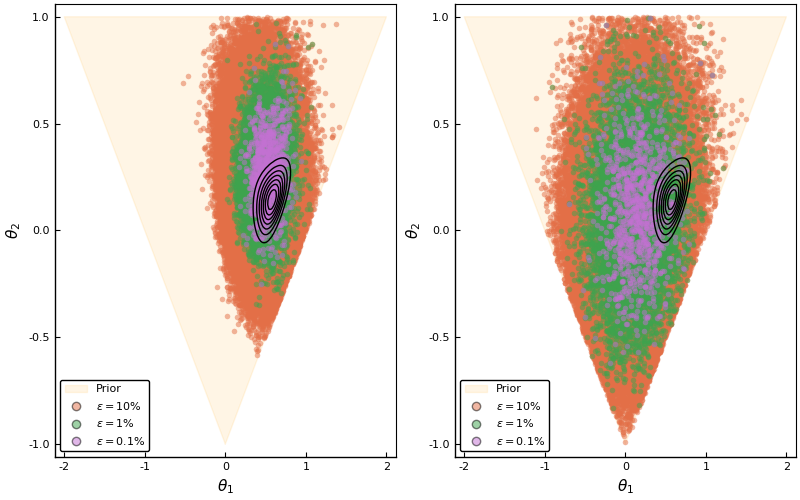
\includegraphics[width=11cm]{images/ABCmodel1_Comparison.png}
        \caption{Comparison of ABC method when using autocovariance
        distance 
        (\textit{left}) versus raw distance (\textit{right}).
        The number of simulations is $N = 10^6$ and different
        thresholds $\epsilon$ are used.}
        \label{fig:calibration1}
    \end{figure}

    \begin{figure}[H]
        \centering
        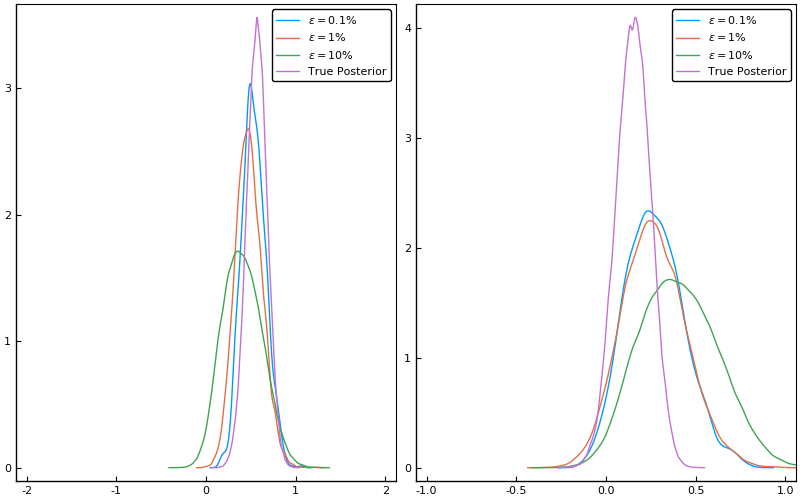
\includegraphics[width=11cm]{images/ABCmodel1_Marginal.png}
        \caption{Comparison of ABC samples with the true posterior
        marginal distribution for $\theta_1$ (\textit{left}) and
        $\theta_2$ (\textit{right}).
        }
        \label{fig:calibration2}
    \end{figure}

% \section{Moving Average}

%
% ---- Bibliography ----
%
% BibTeX users should specify bibliography style 'splncs04'.
% References will then be sorted and formatted in the correct style.
%
\bibliographystyle{apa}
\bibliography{abc}
%
\end{document}
